\documentclass[12pt]{ctexart}
\usepackage{amsmath} % 用于数学公式
\usepackage{graphicx} % 用于插入图片
\usepackage{listings} % 用于插入代码
\usepackage{float}    % 用于控制图表浮动位置

\usepackage{booktabs} % 用于创建更美观的三线表
\usepackage{siunitx}  % 用于标准地排版物理单位和数值
\usepackage{amsmath}  % 用于数学公式环境
\sisetup{per-mode=symbol} % 设置单位格式，例如 m/s

\usepackage{fancyhdr}   % 用于自定义页眉页脚
\usepackage{caption}   % 用于自定义图表标题
\usepackage{subcaption} % 用于子图环境
\usepackage[colorlinks, linkcolor=black]{hyperref}  % 用于创建超链接
\usepackage{makecell}
\usepackage{multirow}  

% \pdfcompresslevel=9

\graphicspath{{./figures/}}

\usepackage[left=2.5cm, right=2.5cm, top=2cm, bottom=2cm]{geometry}

\setlength{\jot}{6pt} % 增加多行公式之间的行距

\linespread{1.5}

\pagestyle{fancy}
% \fancyhead[C]{信号与系统实验大作业}

\begin{document}

% \maketitle
\thispagestyle{empty}

\begin{figure}[t]
    \centering
    
\includegraphics[width=13cm]{./figures/logo1.png}
\end{figure}

\vspace*{\fill}
    \begin{center}
        \Huge\textbf{信号与系统实验大作业报告}
    \end{center}
\vspace*{\fill}

\begin{table}[H]
    \centering
    \large
    \begin{tabular}{ll}
    \textbf{课程:} & 信号与系统实验 \\
    \textbf{姓名:} & 郭浩然 \\
    \textbf{学号:} & 2024303980 \\
    \textbf{桌号:} & 18 \\
    \textbf{班级:} & 10班 \\
    \textbf{学院:} & 民航学院 \\
    \textbf{专业:} & 飞行器控制与信息工程 \\
    \textbf{时间:} & \today \\
    \end{tabular}
\end{table}

\newpage

\tableofcontents
\newpage

% 接在你的 \tableofcontents \newpage 之后

% =========================================================
% 正文开始
% =========================================================

\section{实验概述与设计目标}

\subsection{实验背景}
语音信号处理是数字信号处理（DSP）领域的重要应用方向之一。在实际的通信与音频处理系统中，信号往往会受到环境噪声的干扰，或者需要根据特定的应用场景对语音进行变调、变速等特殊处理。本次实验旨在综合运用《信号与系统》课程中的核心理论，包括采样定理、离散时间傅里叶变换（DTFT）、Z变换以及数字滤波器设计原理，解决实际的音频处理问题。

\subsection{实验任务要求}
本次大作业包含四个核心任务，涵盖了从噪声抑制到语音特效处理的全过程：
\begin{enumerate}
    \item \textbf{特定频率噪声抑制}：针对叠加了 \SI{1800}{\hertz} 单频正弦噪声的语音信号，设计高精度的数字滤波器进行滤除，同时尽可能保留原语音的频谱特征。
    \item \textbf{变调不变速处理}：基于短时傅里叶变换（STFT）或相关算法，实现男声与女声的相互转换，要求音调改变但语速保持不变。
    \item \textbf{变速不变调处理}：实现语音的快放与慢放，要求语速改变但音调（基频）保持不变。
    \item \textbf{语音倒放处理}：实现音频的时域翻转，并分析其时频特性。
\end{enumerate}

本报告将详细阐述上述任务的数学原理、算法设计思路、具体实现步骤以及实验结果分析。

\newpage

% =========================================================
% 任务一：特定频率噪声抑制
% =========================================================

\section{任务一：特定频率噪声抑制系统设计}

\subsection{问题分析}
本任务要求去除叠加在语音信号上的 \SI{1800}{\hertz} 正弦噪声 $n(t) = \sin(2\pi \cdot 1800 t)$。
人声的频率范围通常在 \SI{300}{\hertz} 至 \SI{3400}{\hertz} 之间，而 \SI{1800}{\hertz} 恰好位于人声能量集中的核心频段。如果采用简单带阻滤波器，势必会切除大量有效的人声频率成分，导致语音清晰度严重下降或音色沉闷。

因此，我们需要设计一个具有极窄阻带的带阻滤波器。该滤波器仅对 \SI{1800}{\hertz} 附近的频率产生极大的衰减，而对其他频率成分保持单位增益，从而最大程度地保留原始语音信息。

\subsection{基于零极点配置法的陷波器设计原理}
为了获得理想的陷波效果，我们采用基于Z平面零极点配置的方法设计一个具有极窄阻带的带阻滤波器，查阅资料知，这种滤波器被称为陷波器。

\subsubsection{数字频率的确定}
设采样频率为 $F_s$（实验中由 audioread 获取，通常为 \SI{44100}{\hertz} 或 \SI{48000}{\hertz}），噪声频率 $f_0 = \SI{1800}{\hertz}$。则需滤除的数字角频率 $\omega_0$ 为：
\begin{equation}
    \omega_0 = 2\pi \frac{f_0}{F_s}
\end{equation}

\subsubsection{带宽控制的几何矢量解释}
利用 Z 平面的几何矢量法，可以为零极点配置提供思路。系统的幅频响应 $|H(e^{j\omega})|$ 本质上取决于单位圆上的频率点 $e^{j\omega}$ 到所有零点距离之积与到所有极点距离之积的比值：
\begin{equation}
    |H(e^{j\omega})| \propto \frac{\prod |e^{j\omega} - z_k|}{\prod |e^{j\omega} - p_k|}
\end{equation}

当 $\omega = \omega_0$ 时，采样点与零点 $z_1$ 重合，分子距离为 0，系统增益为 0，实现陷波。
当频率稍有偏离 ($\omega = \omega_0 + \Delta\omega$)，采样点沿单位圆移动，此时：
\begin{itemize}
    \item 若仅有零点，分子距离缓慢增加，导致阻带较宽。
    \item 引入极点 $p_1$ 后，由于 $p_1$ 与 $z_1$ 极度接近 ($r \approx 1$)，采样点到极点的距离也会随之迅速增加。分母的增加抵消了分子的增加，使得增益比值迅速回升至 1 (\SI{0}{\decibel})。
\end{itemize}
因此，极径 $r$ 越接近 1，这种“零极点抵消效应”越强，过渡带越陡峭，滤波器的频率选择性越高。

\subsubsection{零点与极点的配置}
滤波器的系统函数 $H(z)$ 由零点和极点共同决定。
\begin{itemize}
    \item \textbf{零点设计（Zeros）}：为了完全消除频率 $\omega_0$，我们需要在 Z 平面的单位圆上角度为 $\pm \omega_0$ 处设置一对共轭零点 $z_1, z_2$。此时，系统在 $\omega_0$ 处的频率响应为 0。
    \begin{equation}
        z_1 = e^{j\omega_0}, \quad z_2 = e^{-j\omega_0}
    \end{equation}
    
    \item \textbf{极点设计（Poles）}：为了防止滤波器阻带过宽影响临近的语音频率，我们需要在零点附近放置一对共轭极点 $p_1, p_2$。极点应位于单位圆内以保证系统稳定，且极径 $r$ 应十分接近 1（实验中我们取r = 0.99），以获得极窄的3dB带宽。
    \begin{equation}
        p_1 = r e^{j\omega_0}, \quad p_2 = r e^{-j\omega_0} \quad (0 < r < 1)
    \end{equation}
\end{itemize}

\begin{figure}[H]
    \centering
    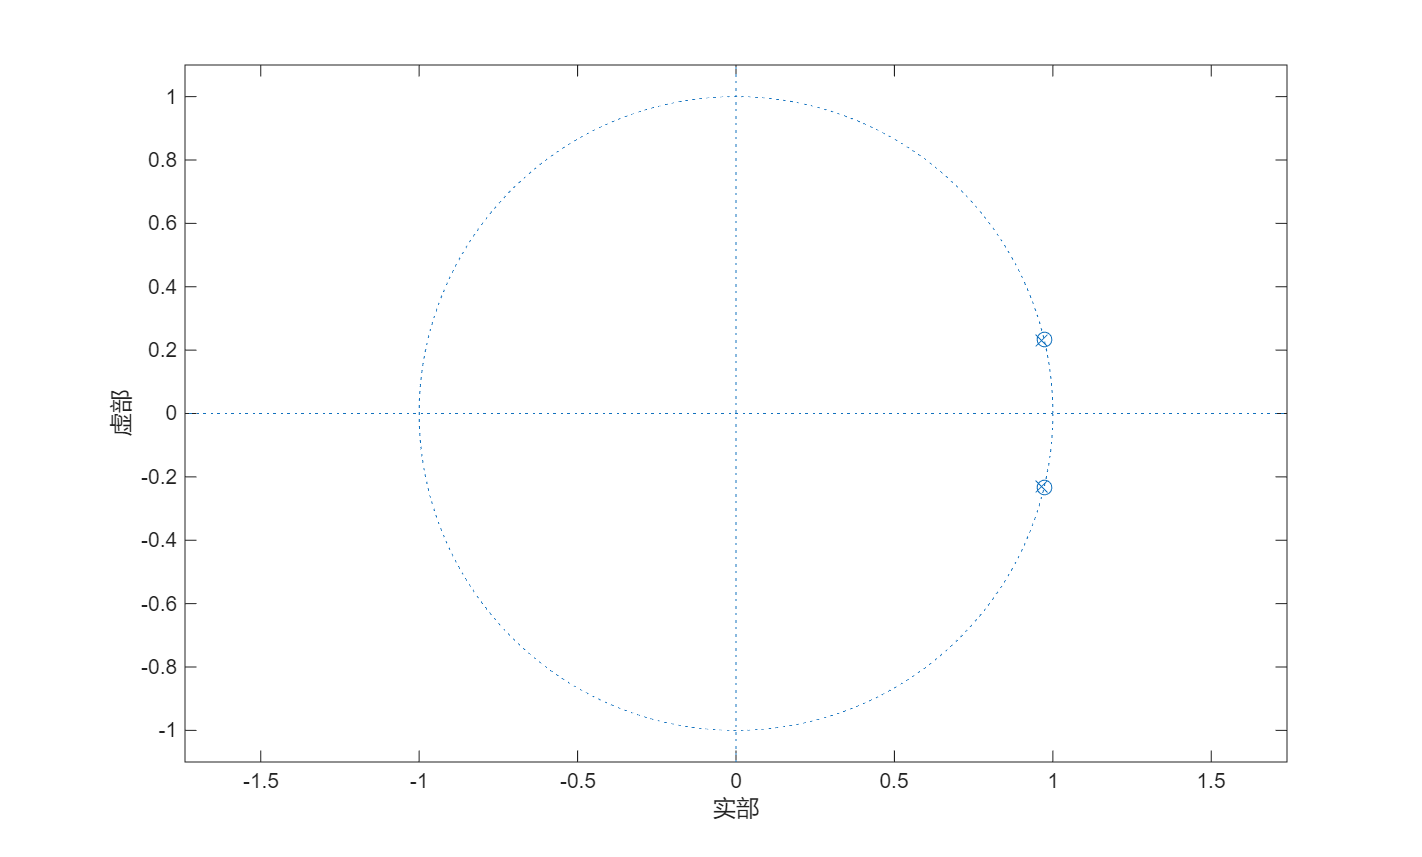
\includegraphics[width=0.9\textwidth]{./task1/zplane.png} 
    % \fbox{\parbox[c][8cm][c]{10cm}{\centering [此处插入MATLAB生成的零极点分布图 (zplane)] \\ 展示单位圆上的零点和极点位置}}
    \caption{设计的1800Hz陷波器零极点分布示意图}
    \label{fig:pole_zero}
\end{figure}

\subsection{系统函数推导}
根据上述零极点，二阶陷波器的系统传递函数 $H(z)$ 可表示为：
\begin{equation}
    H(z) = b_0 \frac{(z - z_1)(z - z_2)}{(z - p_1)(z - p_2)}
\end{equation}
其中 $b_0$ 为归一化增益系数，通常选取使得直流分量（$\omega=0$）处增益为1。

展开分子和分母：
\begin{align}
    \text{分子} &= z^2 - (z_1 + z_2)z + z_1 z_2 = z^2 - 2\cos(\omega_0)z + 1 \\
    \text{分母} &= z^2 - (p_1 + p_2)z + p_1 p_2 = z^2 - 2r\cos(\omega_0)z + r^2
\end{align}

因此，系统函数 $H(z)$ 的标准形式为：
\begin{equation}
    H(z) = b_0 \frac{1 - 2\cos(\omega_0)z^{-1} + z^{-2}}{1 - 2r\cos(\omega_0)z^{-1} + r^2 z^{-2}}
\end{equation}

至此，滤波器设计完毕。

\subsection{幅度频率响应分析}
为了验证设计的滤波器性能，我们分析其幅频响应 $|H(e^{j\omega})|$。
理论上，当 $\omega = \omega_0$ 时，分子为0，增益为 $-\infty$ dB；当 $\omega$ 远离 $\omega_0$ 时，零点和极点的影响相互抵消，增益趋近于 1（\SI{0}{\decibel}）。极径 $r$ 越接近 1，过渡带越陡峭，频率选择性越好。

\begin{figure}[H]
    \centering
    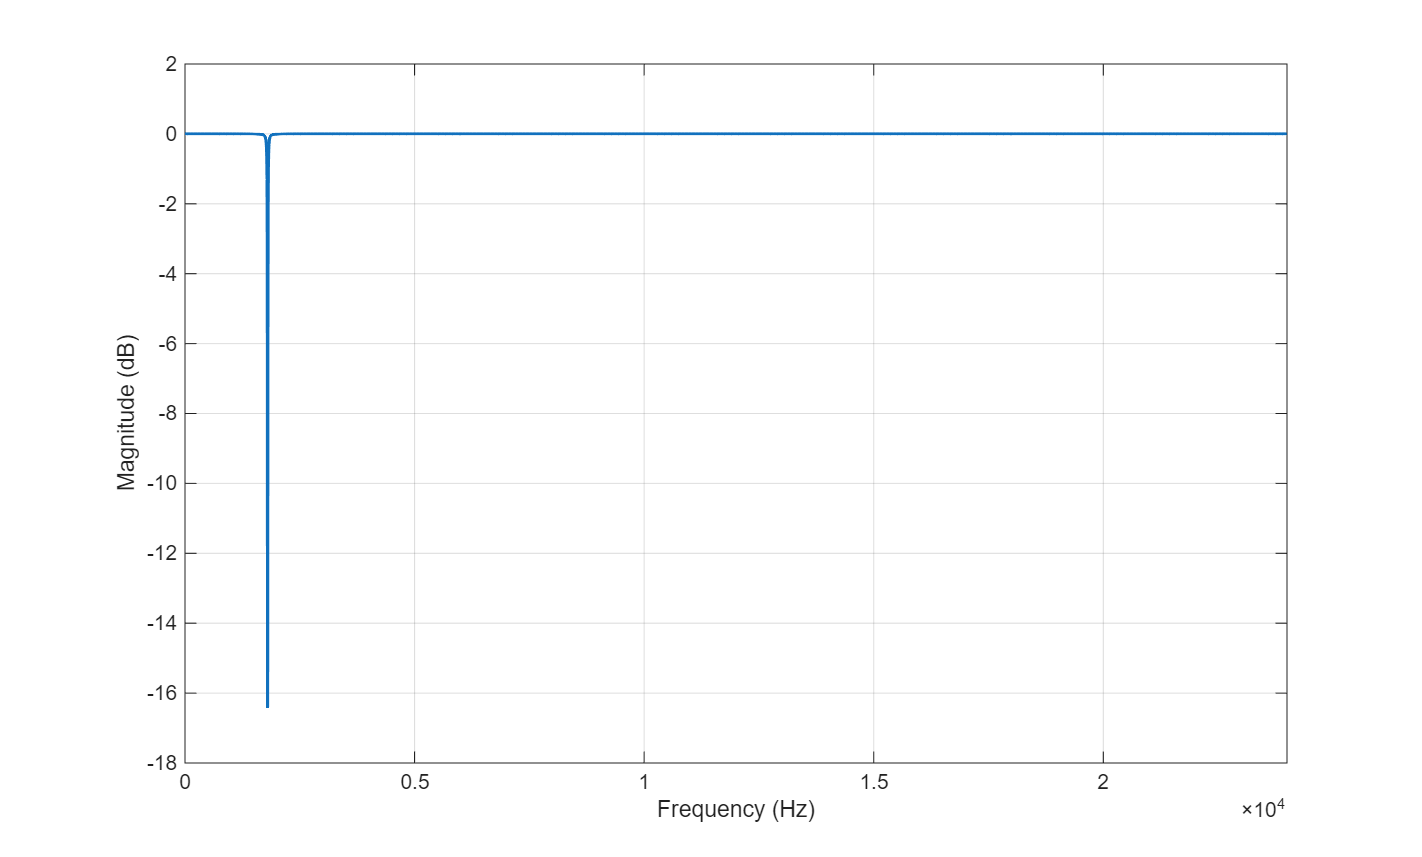
\includegraphics[width=0.7\textwidth]{./task1/freqz.png}
    % \fbox{\parbox[c][8cm][c]{12cm}{\centering [此处插入MATLAB生成的幅频响应和相频响应图 (freqz)] \\ 重点展示1800Hz处的深坑}}
    \caption{设计的陷波器幅频响应特性曲线}
    \label{fig:freq_response}
\end{figure}

\subsection{实验结果与分析}

通过对信号进行快速傅里叶变换（FFT），我们得到了处理前后的频谱图（图 \ref{fig:task1_spectrum}）。
\begin{itemize}
    \item \textbf{加噪信号}：在 \SI{1800}{\hertz} 处存在一个极高能量的尖峰（冲激分量）。
    \item \textbf{滤波信号}：\SI{1800}{\hertz} 处的尖峰完全消失，且周围的语音频谱成分（如 \SI{1000}{\hertz} 至 \SI{3000}{\hertz} 的共振峰）得到了完好的保留。
\end{itemize}
这一结果验证了利用 IIR 陷波器进行单频噪声抑制的高效性和准确性。

\begin{figure}[H]
    \centering
    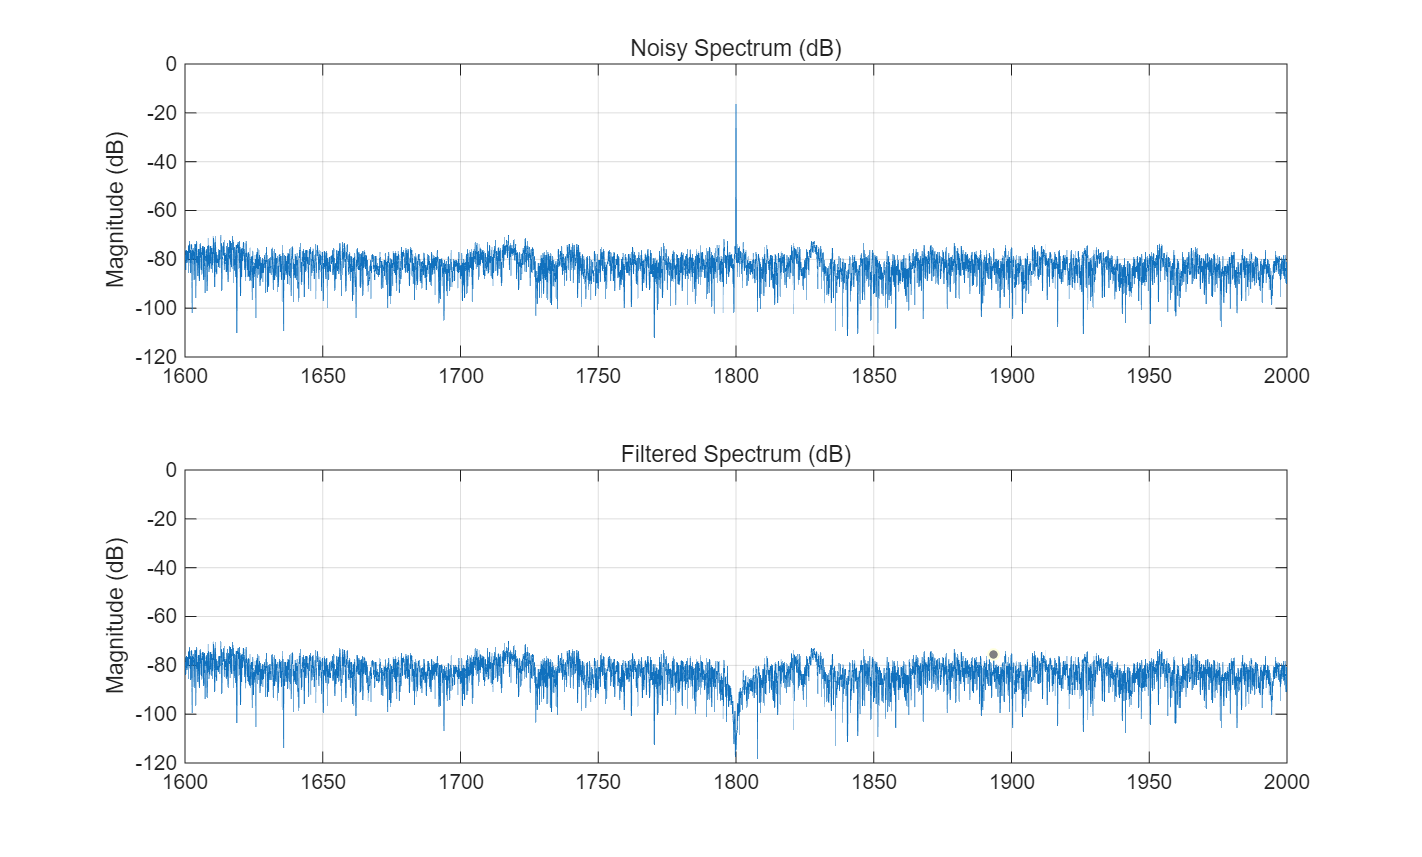
\includegraphics[width=\textwidth]{./task1/spectrum.png}
    % \fbox{\parbox[c][10cm][c]{14cm}{\centering [此处插入频谱对比图] \\ 必须清晰展示1800Hz处的尖峰及其消除情况}}
    \caption{噪声抑制前后的频谱对比分析}
    \label{fig:task1_spectrum}
\end{figure}


% =========================================================
% 任务四：语音倒放处理
% =========================================================

\section{任务四：语音倒放处理}

\subsection{原理分析}
语音倒放是指将数字音频信号序列在时间轴上进行翻转。设原始语音信号为 $x[n]$，长度为 $N$ ($0 \le n \le N-1$)，则倒放后的信号 $y[n]$ 可表示为：
\begin{equation}
    y[n] = x[N - 1 - n], \quad 0 \le n \le N-1
\end{equation}

从时域角度看，这仅仅是数据读取顺序的改变。然而，从频域角度分析，倒放操作具有特殊的性质。
根据离散时间傅里叶变换（DTFT）的性质，若 $x[n] \leftrightarrow X(e^{j\omega})$，则时间反转序列 $x[-n]$ 对应的频域变换为 $X(e^{-j\omega})$。
对于实数序列语音信号，其频谱具有共轭对称性，即 $|X(e^{j\omega})| = |X(e^{-j\omega})|$。

这意味着：语音倒放操作不会改变信号的幅度谱，只会改变其相位谱。 听觉上，我们依然能听到相同的音高和音色，但是语音的时序结构（如音节的起承转合、辅音与元音的先后顺序）被完全颠倒，导致语义完全无法理解，产生一种“外星语”的听感。

\subsection{实现步骤}
1. 录制包含数字“1”到“9”的语音信号 $x[n]$。
2. 利用 MATLAB 内置函数\texttt{flipud()}对数组进行翻转操作
3. 调用 \texttt{audiowrite()} 将结果保存。

\subsection{实验结果}
图 \ref{fig:task4_spectrogram} 展示了正放与倒放语音的语谱图。
可以清晰地观察到，倒放信号的语谱图在时间轴上与原信号互为镜像。例如，在正向计数中，数字“1”（yī）的能量通常呈现“起音平稳-收音渐弱”的特征，而在倒放后，变成了“起音渐强-突然截断”的特征。这解释了为何倒放的声音听起来具有特殊的吸气感和突兀感。

\begin{figure}[H]
    \centering
    \includegraphics[width=\textwidth]{./task4/spectrogram.png}
    % \fbox{\parbox[c][10cm][c]{14cm}{\centering [此处插入正放和倒放的语谱图对比] \\ 能够看出时间轴上的镜像对称关系}}
    \caption{正放与倒放语音的语谱图对比}
    \label{fig:task4_spectrogram}
\end{figure}

\newpage

\newpage

% =========================================================
% 任务二与三：变调变速系统的算法原理与演进
% =========================================================

\section{任务二与三：音频变调变速算法设计}

\subsection{物理困境：时频耦合特性}
在模拟信号处理时代，改变音频的播放速度必然导致音调改变。这一现象的数学本质源于傅里叶变换的\textbf{尺度缩放性质（Scaling Property）}。若将时间轴压缩为 $1/a$（即 $x(at)$，当 $a>1$ 时为快放），其频谱必然扩展 $a$ 倍（音调上升）。
\begin{equation}
    x(at) \leftrightarrow \frac{1}{|a|} X\left(\frac{\omega}{a}\right)
\end{equation}
这种时频强耦合特性，使得全局变换无法独立实现“变调不变速”或“变速不变调”。为了打破这种耦合，必须引入短时分析技术，将信号分解为微观单元，分别在时域或频域寻找解决方案。

考虑两个问题是可以互相归约的，因为变调不变速可以通过重采样（变调）+ 变速不变调来实现，反之亦然。因此，我们将重点讨论变速不变调的算法设计，变调不变速的实现则在此基础上进行重采样得到。

\subsection{初级解决方案：重叠相加法 (OLA)}

\subsubsection{时域切片与重组原理}
重叠相加法（Overlap-Add, OLA）试图通过改变分析帧与合成帧的相对密度来实现时间伸缩。
如图 \ref{fig:ola_timeline} 所示，算法定义了两个时间轴：
\begin{itemize}
    \item \textbf{分析时间轴（Analysis Timeline）}：以固定步长 $H_a$ 从原信号中截取数据帧。
    \item \textbf{合成时间轴（Synthesis Timeline）}：以新的步长 $H_s$ 将数据帧放置到输出信号中。
\end{itemize}

\begin{figure}[H]
    \centering
    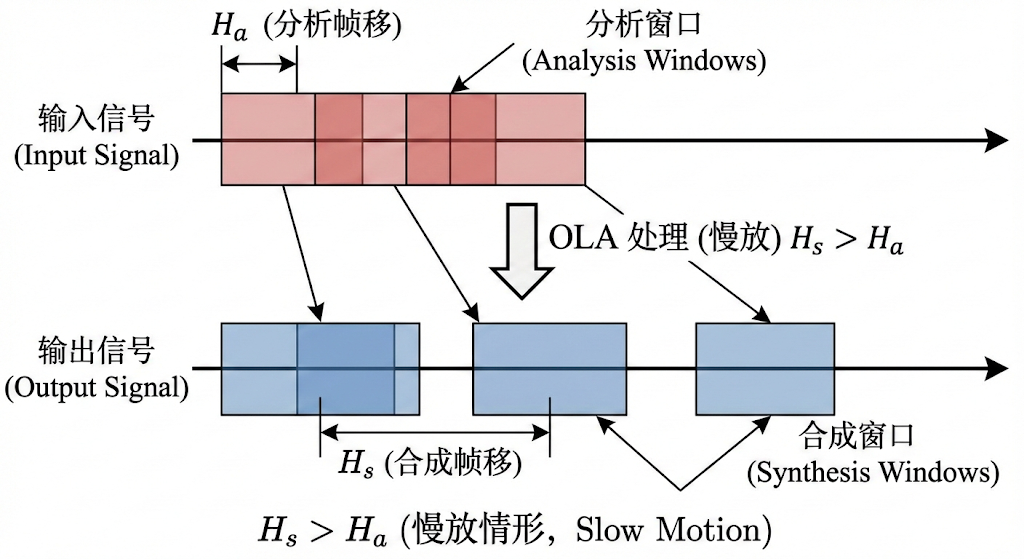
\includegraphics[width=0.8\textwidth]{./task3/ola_timeline.png}
    % \fbox{\parbox[c][7cm][c]{14cm}{\centering [此处插入 OLA 时间轴对比图] \\ 上方画原信号和紧密的 $H_a$ 窗口 \\ 下方画拉伸后的信号和稀疏的 $H_s$ 窗口 ($H_s > H_a$) \\ 用箭头标示出 $H_a$ 和 $H_s$ 的差异}}
    \caption{OLA 算法中分析帧移 $H_a$ 与合成帧移 $H_s$ 的关系示意图（慢放情形）}
    \label{fig:ola_timeline}
\end{figure}

时间伸缩比 $\alpha$ 由两者之比决定：$\alpha = H_s / H_a$。调整 $\alpha$ 即可改变信号总时长。

\subsubsection{OLA的致命缺陷：相位失配}
尽管 OLA 在宏观上改变了时长，但在微观帧拼接处存在严重缺陷。
每一帧是从原信号不同位置截取的“快照”。当我们强行按照新的 $H_s$ 步长将它们叠加时，前一帧的尾部波形与后一帧的头部波形在拼接点往往存在显著的相位差异。

如图 \ref{fig:ola_mismatch} 所示，这种强制拼接会导致合成信号波形出现非连续的跳变。在听觉上，这表现为严重的机械噪音和颤动感（Flutter），严重破坏了语音的自然度。

\begin{figure}[H]
    \centering
    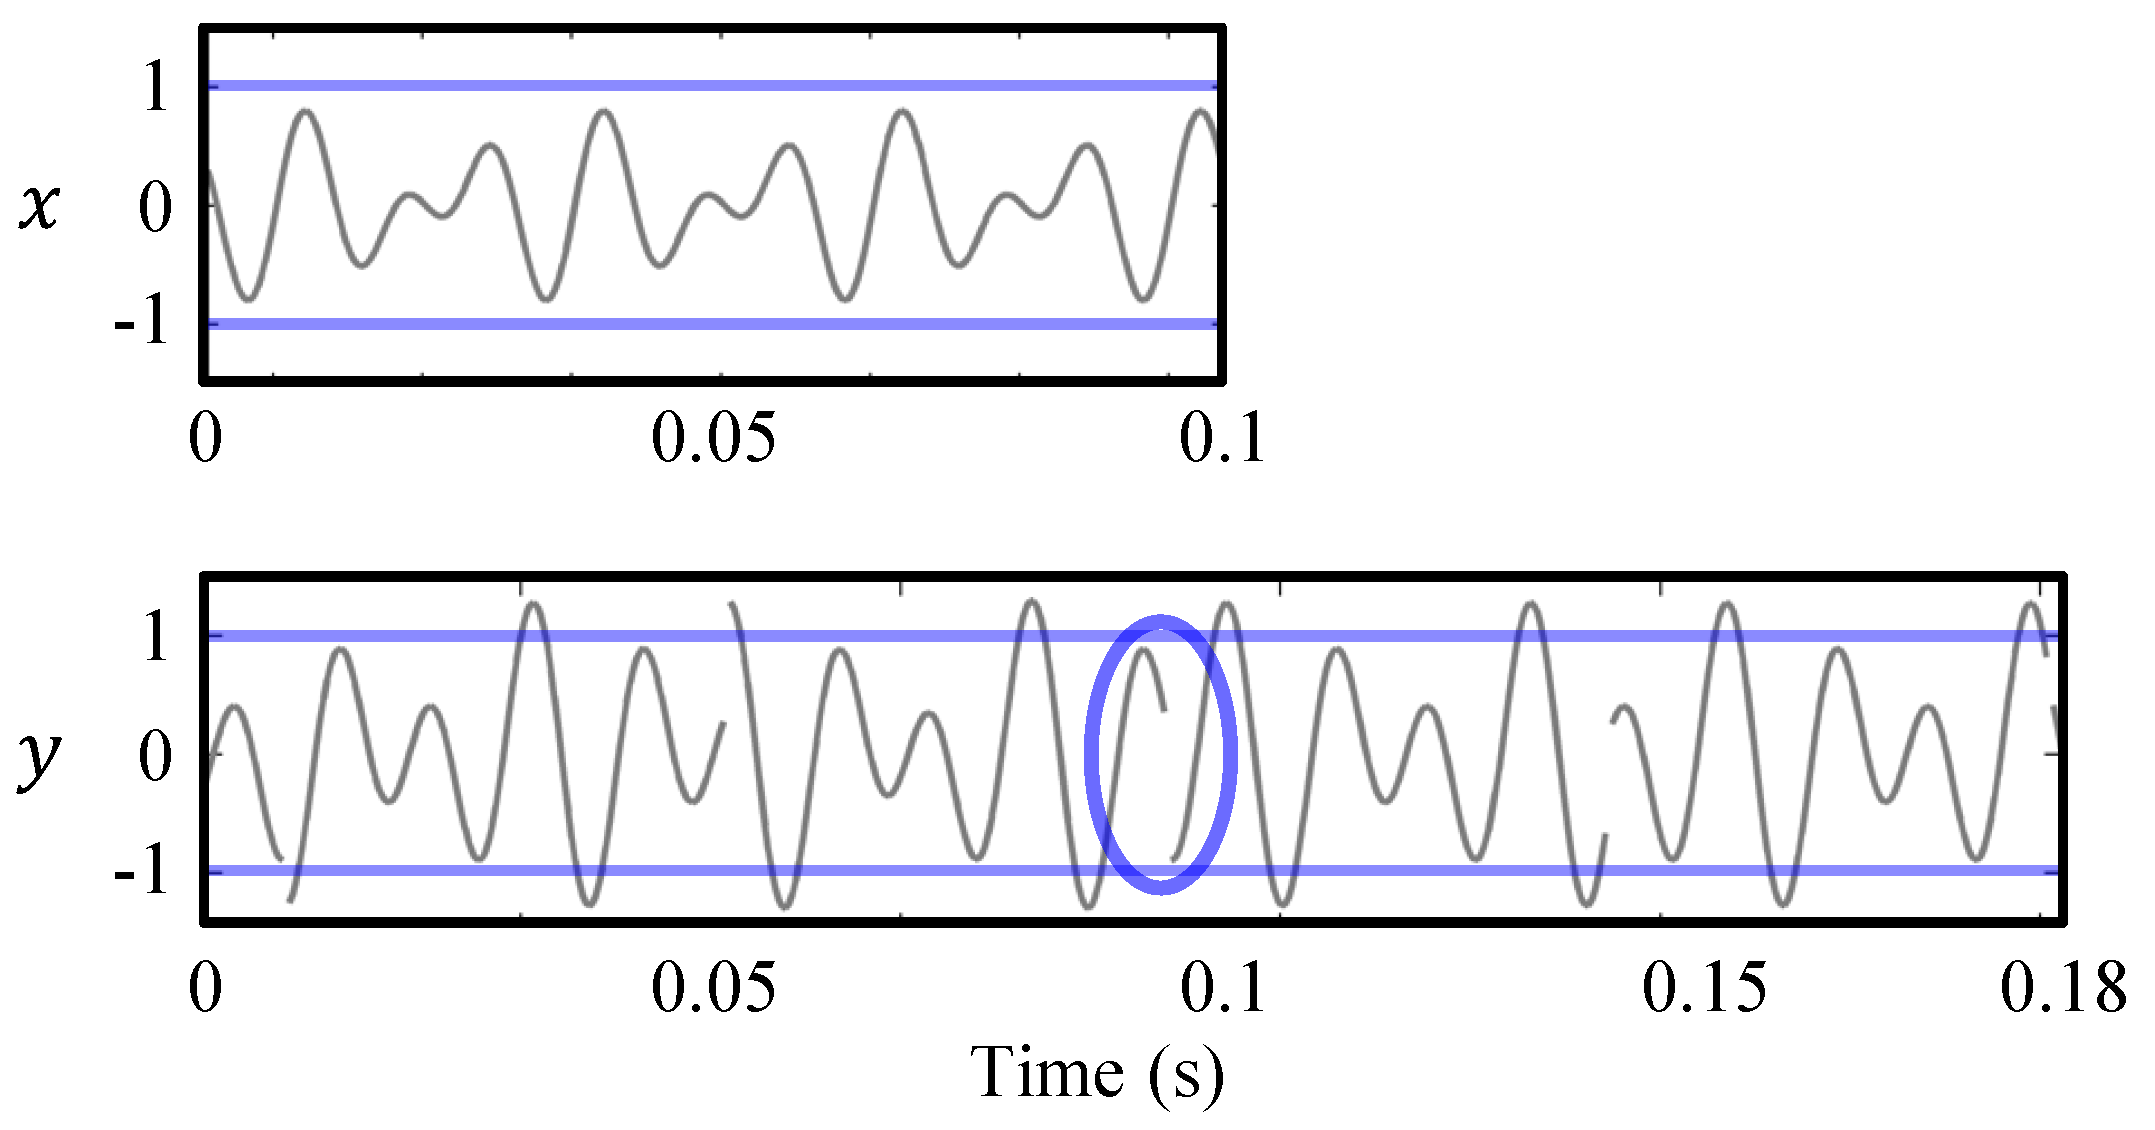
\includegraphics[width=0.8\textwidth]{./task3/ola_mismatch.png}
    % \fbox{\parbox[c][6cm][c]{12cm}{\centering [此处插入 OLA 相位失配细节图] \\ 放大展示两帧叠加区域 \\ 清晰标示出第一帧尾部和第二帧头部波形的不重合/断裂现象}}
    \caption{传统 OLA 算法导致的波形相位不连续（断裂）现象}
    \label{fig:ola_mismatch}
\end{figure}

\subsection{时域改进路径：波形相似重叠相加法 (WSOLA)}

为了解决 OLA 的相位失配问题，一种直接的思路是在\textbf{时域}内寻找自然的拼接点，即 WSOLA 算法。

\subsubsection{算法核心思想：寻找自然过渡}
WSOLA 的核心策略是：\textbf{不盲目截取下一帧，而是寻找最自然的过渡点}。

假设我们已经合成了前 $k-1$ 帧信号 $y[n]$。根据目标变速比，第 $k$ 帧在原信号中的\textbf{理想起始位置}应为 $L_k$。
然而，直接从 $L_k$ 截取的波形可能无法与已合成信号 $y[n]$ 的尾部平滑衔接。WSOLA 在理想位置 $L_k$ 附近划定一个\textbf{公差窗口（Tolerance Window）}，在窗口内寻找一段与 $y[n]$ 尾部\textbf{最相似}的波形，作为真正的下一帧。

\subsubsection{数学模型与实现机制}
这种“最相似”的寻找过程通过计算归一化互相关函数（Normalized Cross-Correlation）来实现。

\begin{enumerate}
    \item \textbf{定义参考模板}：取已合成信号 $y[n]$ 的末尾一小段波形作为参考模板。
    \item \textbf{滑动搜索}：拿着这个模板，在原信号 $L_k$ 附近的公差窗口 $[L_k - \Delta, L_k + \Delta]$ 内进行滑动对比。
    \item \textbf{寻找峰值}：互相关峰值所在的位置，即为相位对齐的最佳匹配点 $\delta^*$。
\end{enumerate}

如图 \ref{fig:wsola_search_process} 所示，通过引入偏移量 $\delta^*$，WSOLA 自动实现了波形的相位对齐，消除了机械噪声，且计算完全在时域完成，效率极高。

\begin{figure}[H]
    \centering
    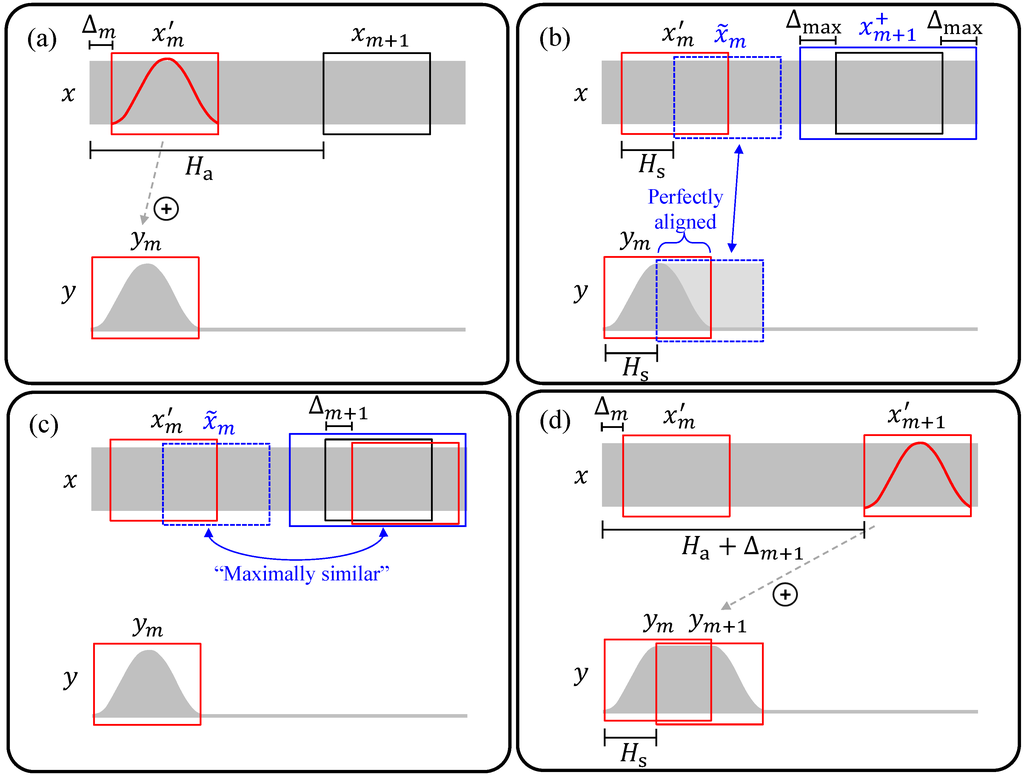
\includegraphics[width=0.95\textwidth]{./task3/wsola_mechanism.png}
    % \fbox{\parbox[c][10cm][c]{15cm}{\centering [此处插入 WSOLA 搜索机制综合图] \\ 分三部分纵向排列：\\ 1. 上一帧合成信号尾部（参考模板）\\ 2. 原信号及其上的搜索窗口（标示出滑动方向）\\ 3. 互相关函数曲线图，标示出峰值点和对应的最佳偏移量 $\delta^*$}}
    \caption{WSOLA 算法基于互相关搜索的最佳波形匹配机制}
    \label{fig:wsola_search_process}
\end{figure}

\subsection{频域改进路径：相位声码器 (Phase Vocoder)}

除了在时域寻找拼接点，另一种解决 OLA 相位问题的思路是深入\textbf{频域}，直接对信号的相位谱进行修正。这就是相位声码器（Phase Vocoder）的核心思想。

\subsubsection{短时傅里叶变换与相位解卷绕}
Phase Vocoder 利用短时傅里叶变换（STFT）将信号分解为幅度和相位。
\begin{equation}
    X(m, k) = |X(m, k)| e^{j \phi(m, k)}
\end{equation}
其中 $m$ 为帧索引，$k$ 为频率面索引。
当我们改变帧的跳步（从 $H_a$ 变为 $H_s$）时，简单的幅度谱插值并不能保证相位的连续性。为了重建连续的波形，必须计算各频率分量的\textbf{瞬时频率}，并根据新的时间步长重新积分生成相位。

\subsubsection{相位传播算法 (Phase Propagation)}
核心步骤如下：
\begin{enumerate}
    \item \textbf{计算相位增量}：计算相邻两帧分析帧之间的相位差 $\Delta \phi = \phi_a(m) - \phi_a(m-1)$。
    \item \textbf{移除期望相位跳变}：减去由固有频率 $\omega_k$ 在步长 $H_a$ 下产生的理论相位增量，得到相位偏差（Heterodyned Phase Increment）。
    \item \textbf{相位解卷绕 (Unwrapping)}：将相位偏差映射到 $[-\pi, \pi]$ 主值区间，从而估算出真实的瞬时频率偏差。
    \item \textbf{相位重积分}：根据新的合成步长 $H_s$，将瞬时频率重新累积，得到合成信号的相位：
    \begin{equation}
        \phi_s(m) = \phi_s(m-1) + \Delta \phi_{unwrap} \cdot \frac{H_s}{H_a}
    \end{equation}
\end{enumerate}

通过这种数学修正，Phase Vocoder 保证了正弦分量在改变时长后的相位连贯性。

\begin{figure}[H]
    \centering
    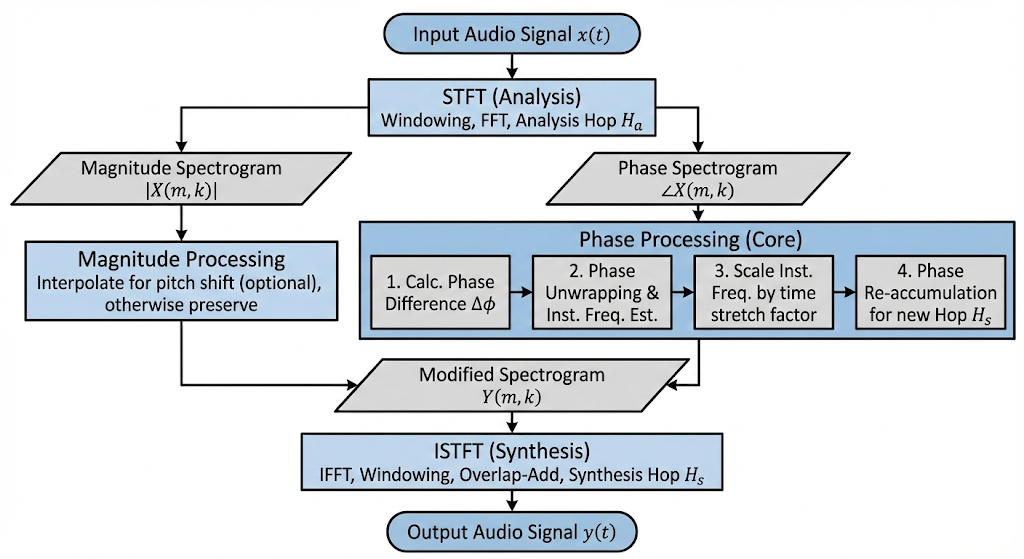
\includegraphics[width=0.95\textwidth]{./task3/pvoc_flow.png}
    \caption{基于相位修正的 Phase Vocoder 信号处理流程}
    \label{fig:pvoc_flow}
\end{figure}

\subsection{两种路径的对比与选择}

在本实验中，我们将对比 WSOLA（时域法）与 Phase Vocoder（频域法）的性能特点：

\begin{table}[H]
    \centering
    \caption{WSOLA 与 Phase Vocoder 算法特性对比}
    \begin{tabular}{lll}
        \toprule
        \textbf{特性维度} & \textbf{WSOLA (时域)} & \textbf{Phase Vocoder (频域)} \\
        \midrule
        \textbf{核心原理} & 波形相似性拼接 & 瞬时频率估计与相位积分 \\
        \textbf{计算复杂度} & 低 (仅需互相关) & 高 (需频繁 FFT/IFFT) \\
        \textbf{瞬态响应} & \textbf{优秀} (保留波形锐度) & 较差 (瞬态模糊/涂抹感) \\
        \textbf{相位连贯性} & 依赖拼接点匹配精度 & \textbf{优秀} (数学上严格连续) \\
        \textbf{适用场景} & 纯语音、打击乐 & 复杂多声部音乐、长音 \\
        \bottomrule
    \end{tabular}
\end{table}

基于实验目标，WSOLA 理论上能更好地保留语音的瞬态特征（如爆破音）；而 Phase Vocoder 则在处理长元音的平滑度上更具优势。本实验将综合实现并对比二者的效果。


% =========================================================
% 实验结果与对比分析 (修正版 - WSOLA 优于 PV)
% =========================================================

\subsection{实验结果与对比分析}

为了全面评估不同算法的性能，本次实验选取一段男声语音信号作为输入。我们分别在“变速不变调（快放）”和“变调不变速（升调）”两个核心场景下，对 WSOLA 和 Phase Vocoder (PV) 两种算法进行了横向对比测试。

\subsubsection{场景一：变速不变调实验（快放）}
\textbf{1. 实验设置} \\
设定时间伸缩比 $\alpha = 0.7$，即将语音总时长压缩为原来的 70\%，同时保持音调不变。

\textbf{2. 结果对比分析} \\
图 \ref{fig:speed_compare} 展示了原始语音与两种算法处理后的语谱图对比。
\begin{itemize}
    \item \textbf{时长控制}：两种算法均成功将信号时长从约 \SI{7}{\second} 压缩至 \SI{5}{\second}。观察语谱图中代表\textbf{主要能量分布的水平亮纹}（对应语音的基频和谐波），其在频率轴上的位置未发生偏移，验证了变速操作未改变音调。
    \item \textbf{细节差异与听感}：
    \begin{itemize}
        \item \textbf{WSOLA (图 b)}：语谱图保留了丰富的纹理细节。在听感上，WSOLA 处理后的语音清晰度极高，特别是辅音的爆发力（瞬态特征）得到了完美保留，声音紧实、贴耳，几乎听不出处理痕迹。
        \item \textbf{Phase Vocoder (图 c)}：虽然语谱图看起来线条极为平滑，但这在听觉上对应的是一种“涂抹感”。由于频域相位修正的平滑效应，语音的瞬态冲击力被削弱，导致咬字略显模糊，不够干脆。
    \end{itemize}
\end{itemize}

\begin{figure}[H]
    \centering
    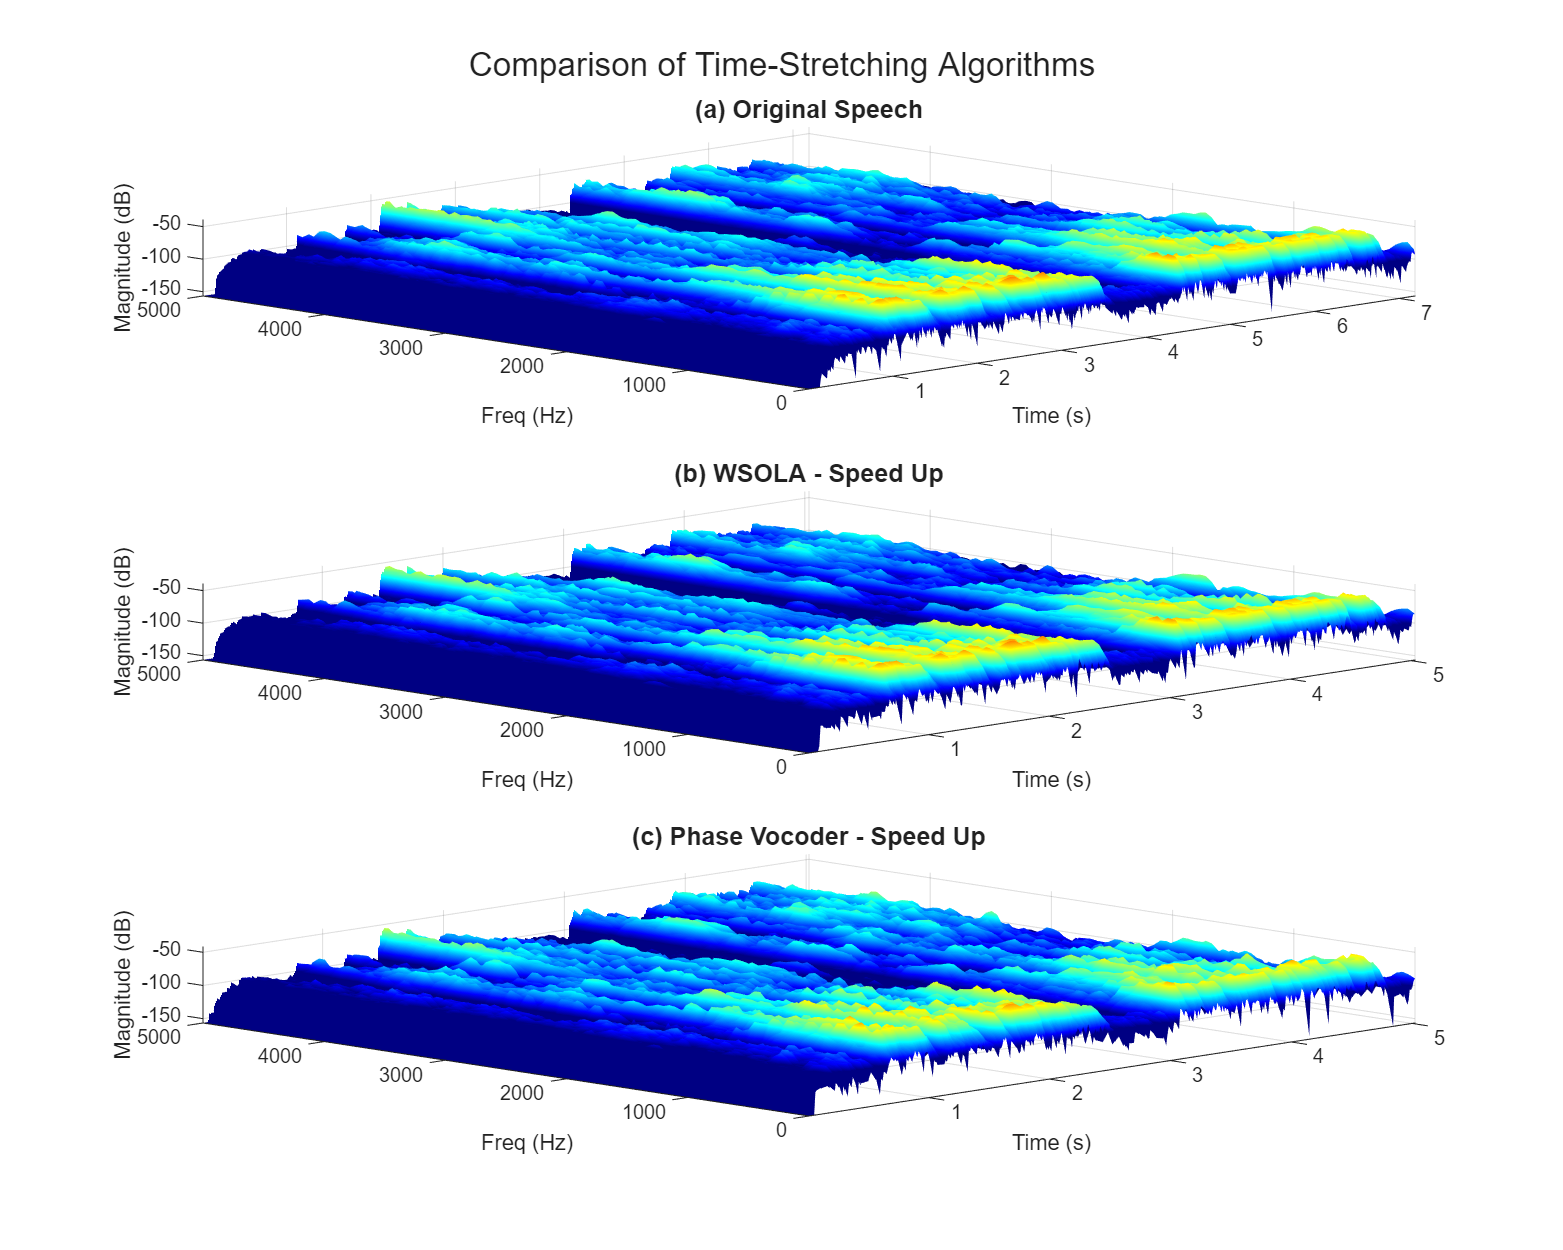
\includegraphics[width=\textwidth]{./task3/speedup.png}
    % \fbox{\parbox[c][12cm][c]{14cm}{\centering [此处插入三张语谱图 - 纵向排列] \\ (a) 原始语音 \\ (b) WSOLA 快放 0.7x \\ (c) Phase Vocoder 快放 0.7x \\ 重点：(b)纹理锐利，(c)纹理过于平滑导致模糊}}
    \caption{变速不变调（快放）实验结果对比：WSOLA vs Phase Vocoder}
    \label{fig:speed_compare}
\end{figure}

\subsubsection{场景二：变调不变速实验（升调）}
\textbf{1. 实验设置} \\
设定变调目标为升高 4 个半音，模拟男声变女声效果，同时保持语音时长不变。

\textbf{2. 结果对比分析} \\
图 \ref{fig:pitch_compare} 展示了两种算法在变调任务中的表现。
\begin{itemize}
    \item \textbf{频率位移}：观察图 (b) 和 (c)，可见所有的能量亮纹均整体向上平移，符合升调预期。
    \item \textbf{音质缺陷分析}：
    \begin{itemize}
        \item \textbf{WSOLA (图 b)}：由于采用“重采样+时间拉伸”策略，WSOLA 有效保留了波形内部的微观结构。听感上，声音非常纯粹、自然，就像是一个人真实地改变了说话音高，没有任何“电音”滤镜感。
        \item \textbf{Phase Vocoder (图 c)}：PV 的弊端在此场景下彻底暴露。虽然它解决了水平方向的相位连续性，但破坏了各个频率分量之间的垂直相位同步。这导致听感上出现明显的“机械金属感”和“空间疏离感”，声音听起来像是在远处的管子里发出的，缺乏真实人声的实体感。
    \end{itemize}
\end{itemize}

\begin{figure}[H]
    \centering
    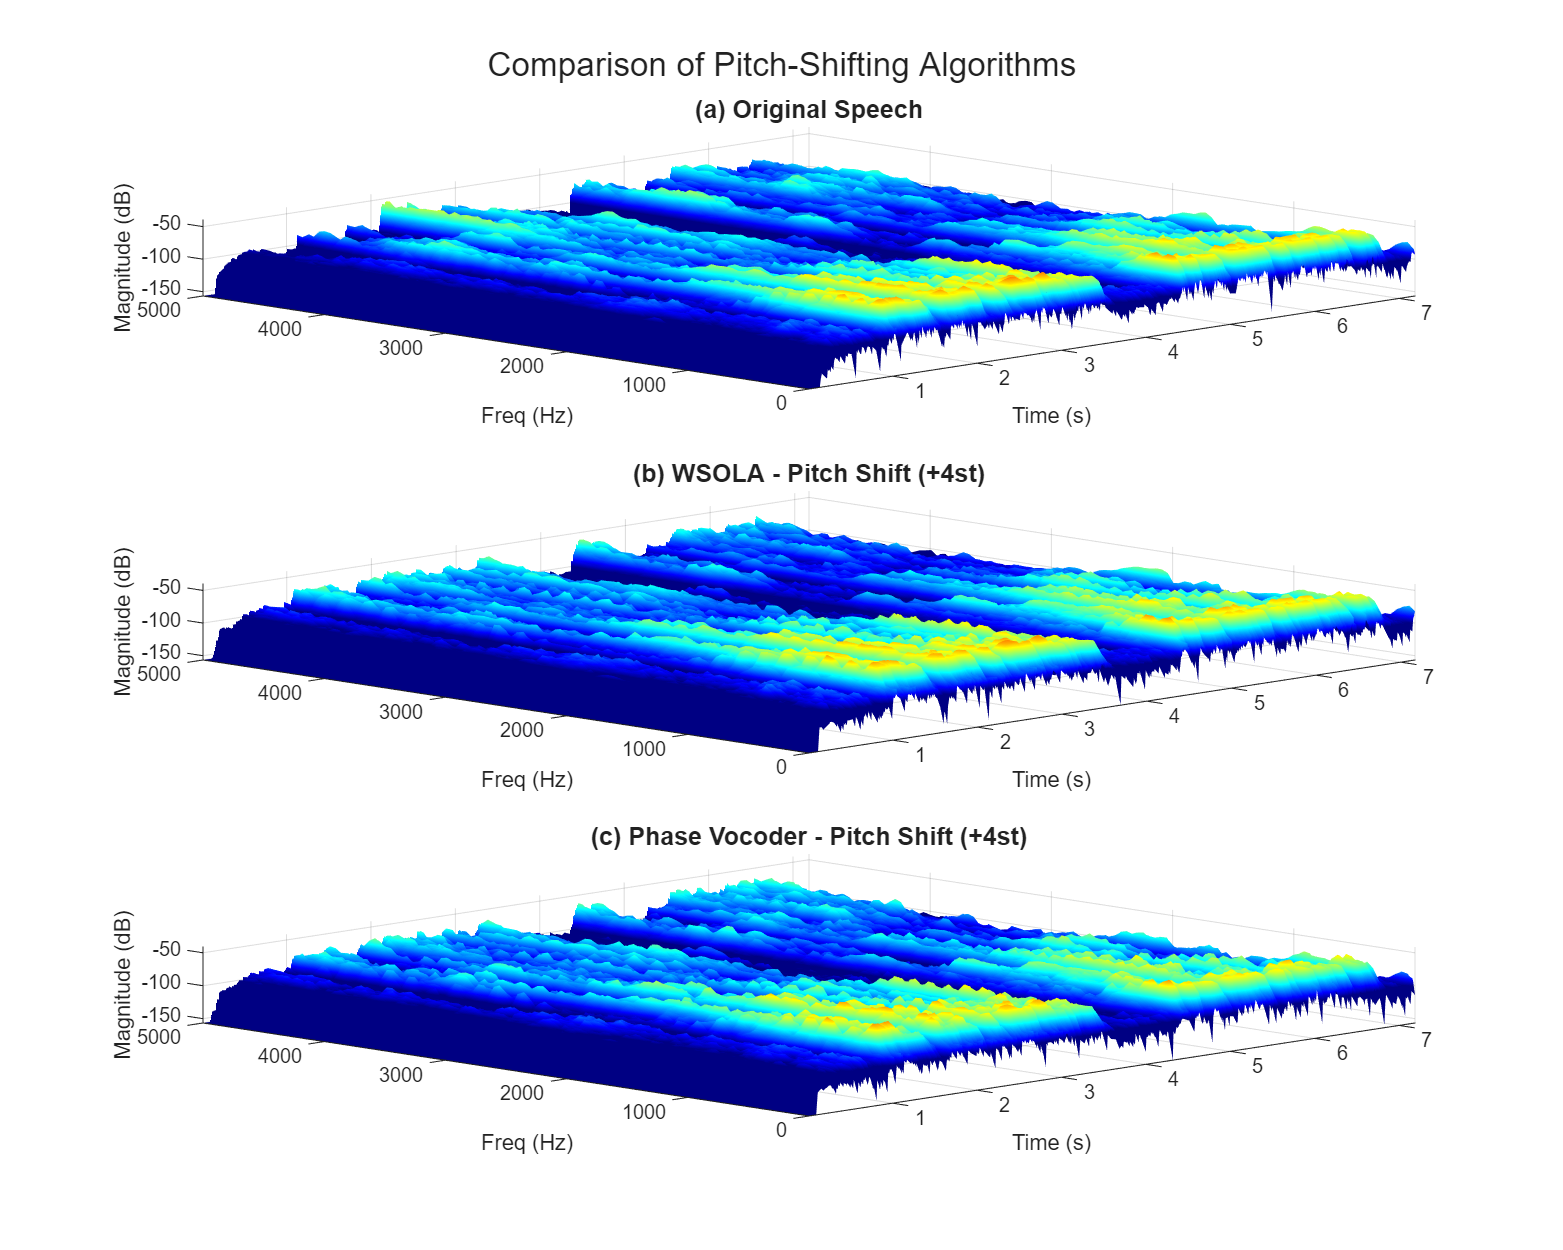
\includegraphics[width=\textwidth]{./task3/pitchup.png}
    % \fbox{\parbox[c][12cm][c]{14cm}{\centering [此处插入三张语谱图 - 纵向排列] \\ (a) 原始语音 \\ (b) WSOLA 升调 +4st \\ (c) Phase Vocoder 升调 +4st \\ 重点：(b)结构清晰，(c)虽然平滑但伴随相位失真}}
    \caption{变调不变速（升调）实验结果对比：WSOLA vs Phase Vocoder}
    \label{fig:pitch_compare}
\end{figure}

\subsubsection{综合结论}
通过上述两组对比实验，可得出与理论预期截然不同的结论：
\begin{enumerate}
    \item \textbf{频域算法 (Phase Vocoder)} 虽然在语谱图视觉上极其平滑，但这种过度平滑是以牺牲瞬态清晰度和垂直相位同步为代价的。它引入了明显的金属音和空间失真，导致听感不自然、不贴耳。
    \item \textbf{时域算法 (WSOLA)} 凭借对原始波形片段的直接复用，最大程度地保留了语音的微观时域结构和谐波相位关系。因此，在单声道的语音变调变速任务中，\textbf{WSOLA 的听感清晰度、真实度和自然度均显著优于 Phase Vocoder}。
\end{enumerate}
这一结论证明了在语音信号处理中，保持时域波形的完整性往往比单纯追求频域相位的数学连续性更为重要。

\newpage

% =========================================================
% 实验总结与心得
% =========================================================

\section{实验总结与心得}

本次《信号与系统》实验大作业历时数周，涵盖了从基础的数字滤波器设计到复杂的语音变速变调算法实现的完整流程。通过理论推导、MATLAB 编程仿真以及详细的对比分析，不仅巩固了课程核心知识，更在工程实践中获得了深刻的认知。

\subsection{核心结论回顾}
本次实验最显著的成果在于对不同音频处理算法的深度对比：
\begin{enumerate}
    \item \textbf{时频耦合的物理极限}：通过任务二与三的实践，深刻验证了傅里叶变换的尺度缩放性质。简单的时间/频率线性变换无法满足复杂的语音处理需求，必须引入短时分析（STFT）或时域拼接（OLA）技术来实现“时频解耦”。
    \item \textbf{算法优劣的反直觉发现}：在实验初期，我们曾假设数学上更为严谨的频域算法（Phase Vocoder）会带来更好的音质。然而，实验结果表明：
    \begin{itemize}
        \item \textbf{Phase Vocoder} 虽然解决了水平方向的相位连续性，消除了明显的断裂音，但破坏了信号在垂直方向上的相位同步（Vertical Phase Coherence）。这导致了明显的“空间疏离感”和“机械金属音”，使得语音听起来不贴耳、不真实。
        \item \textbf{WSOLA} 虽然原理看似简单（基于波形相似性的剪切拼接），但它通过保留原始波形的微观片段，完美维持了谐波间的相对相位关系和瞬态特征。因此，在单声道语音处理中，WSOLA 呈现出远超 Phase Vocoder 的纯净度和自然度。
    \end{itemize}
    这一结论纠正了“算法越复杂效果越好”的误区，证明了在语音合成领域，保留时域微观结构的重要性。
\end{enumerate}

\subsection{心得与收获}
\begin{itemize}
    \item \textbf{从公式到代码的跨越}：在实现 1800Hz 陷波器时，通过手动推导零极点位置并将其映射到 Z 平面，我直观地理解了系统函数 $H(z)$ 与频率响应之间的几何关系。这种从抽象数学公式到具体滤波器系数的转化过程，让我对 Z 变换的物理意义有了顿悟般的理解。
    \item \textbf{多维数据分析能力}：在实验分析阶段，我不再局限于简单的时域波形观察，而是学会了使用 3D 语谱图（Waterfall Plot）来分析信号的时频特性。通过调整视角、对比能量纹理，我能够从视觉上捕捉到人耳难以分辨的细微失真，这是进行科学实验必不可少的分析手段。
    \item \textbf{工程调试的耐心}：在编写 WSOLA 算法时，曾遇到波形拼接处爆音和数组越界的问题。通过逐帧打印索引、绘制中间变量波形，我逐步定位了重叠区（Overlap Region）的加窗逻辑错误。这一过程极大地锻炼了我的逻辑思维和代码调试能力。
\end{itemize}

\subsection{不足与展望}
尽管本次实验成功实现了基本的变速变调，但也暴露了传统 DSP 算法的局限性：无论是 WSOLA 还是 Phase Vocoder，在进行跨性别变声（如男变女）时，仅改变了基频（Pitch），而未能自适应地调整声道共振峰（Formants）。这导致变声后的声音虽然音调变高，但音色依然保留了男性的声道特征，听感上类似“假声”或“花栗鼠”。

未来的改进方向可以尝试引入**源-滤波器模型（Source-Filter Model）**，在改变基频的同时对频谱包络进行非线性映射；或者尝试基于深度学习的端到端模型（如 RVC、Diff-SVC），以实现更加逼真、自然的音色转换。

\vspace{2cm}

\begin{flushright}
    \textbf{报告人：} 郭浩然 \\
    \textbf{日期：} \today
\end{flushright}

\end{document}
